O problema de enovalemento da proteína é a questão fundamental de como a sua sequência de aminoácidos
no plano se transforma em uma estrutura atômica tridimensional. Esta questão é essencial, pois
um melhor entendimento dessa situação pode levar ao desenvolvimento de novos remédios e também
uma melhora no combate de doenças. No entanto, continua sendo um grande desafio obter
uma estrutura estável da proteína a partir da sequência de aminoácidos.
Recentemente, alguns estudos \cite{Rocklin2017} desenvolveram novas proteínas usando o softaware
\textit{Rosetta}, que modela estruturas macromolecures. Existem alguns problemas no
desenvolvimento usando tal software, como proteínas modeladas que não são tão
estáveis sobre o processo de proteólise, que é a quebra da proteína em pedaços
menores. Pode-se contornar este problema através do uso de outras ferramentas avançadas, como
as encontradas em aprendizado de máquinas e análise topológica de dados.

Neste capítulo estudamos a estabilidade de proteínas sobre um score proposto
em \cite{Rocklin2017} utilizando imagens de persistência \cite{Adams2017}, descritas
no Capítulo \ref{chapter:miscel}, e vários algoritmos de aprendizado de máquinas
implementados em \cite{scikit-learn}. Mais detalhes são dados na Seção \ref{sec:stabprot}

Por outro lado podemos estudar a perfomance de algoritmos para modelagem computacional e
análise estrutural de proteínas, como \textit{Rosetta} e \textit{Amber}.
Em \cite{Rubenstein2018}, ambos os softwares sõa comparados em relação a proteína-energia.
Para uma proteína específica, eles geraram milhares de moléculas similares e calcularem
a raíz do erro quadrático médio em relação a proteína original.
Após isso, eles analisaram as móleculas de falso mínimo. Dada uma lista de proteínas
simuladas, elas são ranqueadas de acordo com suas energias normalizadas. Uma molécula
simulada é uma falsa mínima se está no top $10$ das moléculas no ranking a seu
RMSD é maior do que $5$. Eles observaram que o software \textit{Rosetta} gerou mais
proteínas de falso mínimo do que o \textit{Amber}. Na Seção \ref{sec:predrmsd}
analisamos a estrutura das proteínas dadas pelo \textit{Rosetta} utilizando ciclos ótimos
\cite{Escolar2015}, imagens de persistência \cite{Adams2017}, VAE's \cite{kingma2013} e
diversos algoritmos de machine learning utilizando o sklearn \cite{scikit-learn}. Nós
tentamos prever e apresentar uma nova função para ajudar o \textit{Rosetta} no seu
passo de otimização quando simulando novas moléculas.

\section{Estudando a estabilidade - Proteínas I}\label{sec:stabprot}

O desenvolvimento de novas moléculas através de softwares acelerou o estudo de 
novas estruturas atômicas e suas propriedades. No entanto, fica cada vez mais díficil
verificar experimentalmente se uma proteína modelada computacionalmente é estável ou não,
pois por várias vezes existem milhares ou dezenas de milhares de moléculas, dificultando
a experimentação no laboratório devido ao grande número e o seu custo relacionado.

Em \cite{Rocklin2017} eles apresentam um novo método de desenvolvimento de proteínas
com o auxílio de algoritmos de aprendizado de máquinas. Para cada round de desenvolvimento
de proteínas, eles selecionam apenas algumas para testar a estabilidade no laboratório e 
estudar o que precisa ser modificado na estrutura da molécula para o próximo round de 
experimentos computacionais. Nesta seção apresentamos um método que utiliza 
análise topológica de dados para selecionar as moléculas com resultados similares. Porém, 
utilizando homologia persistente obtemos outra informações geométricas da proteína, que pode
auxiliar no desenvolvimento e aprimoramento em cada round de experimentos. Por exemplo, as informações 
dos buracos e cavidades, que podem ser obtidas com a homologia persistente, nos dizem o quão hidrofóbica 
ou hidrofílica uma proteína é. \cite{Jamadagni2011} 

\subsection{A estabilidade da proteína}
Dada uma proteína modelada, podemos medir a sua estabilidade da seguinte maneira. Primeiro,
deposita-se várias cópias da proteína sobre uma célula de levedura, para várias céulas. Então cada 
célula é geneticamente fundida à uma tag de expressão que pode ser tabelada com fluorescência. 
Assim, as células são encubadas com diversas concentrações diferentes de enzimas proteolíticas. 
A quantidade de enzimas utilizadas para quebrar metade das proteínas depositadas na levedura
são então gravadas e vão dar o score de estabilidade da proteína. Se um valor baseado 
nessa soma das concentrações for maior que 1, dizemos que a proteína é estável, caso contrário
dizemos que ela é instável. Podemos ver na Figura~\ref{fig:yeast_cell} o processo de quebra
das cópias da proteína. Mais detalhes podem ser vistos em \cite{Rocklin2017}.

\begin{figure}
    \centering
    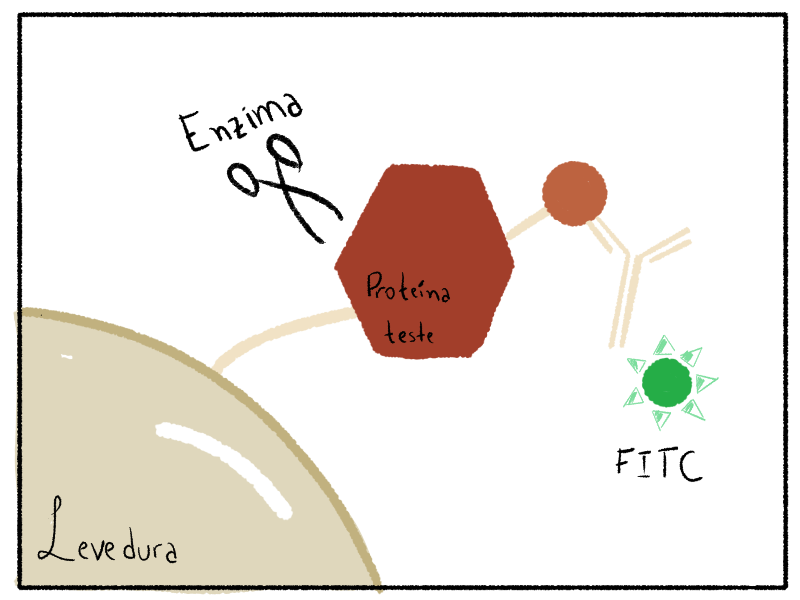
\includegraphics[width=.8\textwidth]{images/yeast_cell.png}
    \caption{Processo de quebra de uma cópia da proteína sobre a superfície de uma 
            célula de levedura.}
    \label{fig:yeast_cell}
    \fautor
\end{figure}

\subsection{Prevendo a estabilidade}
O conjunto de proteínas utilizado contém 12927 moléculas para o treinamento e 
3232 proteínas para o teste. No conjunto de treinamento existem 2210 proteínas 
estáveis (com score maior do que 1) enquanto que no conjunto de treinamento 
existem 305 moléculas estáveis. 

Cada proteína tem 110 propriedades associadas, ou seja, valores numéricos,
que vão desde área de superfície não acessível (relacionada à hidrofobicidade
da proteína) a potenciais coulombianos.  

Os autores de \cite{Rocklin2017} desenvolveram um algoritmo para prever a estabilidade
da proteína e selecionar as melhores moléculas para testes em laboratório. Eles usaram 
o algoritmo de árvore de decisões \textit{Random forest} para treinar mais de 12000
proteínas e prever seu score de estabilidade. Foi treinado um regressor com o erro quadrático
médio (MSE em inglês) para a minimização. Os resultados são dados em relação à raíz do erro quadrático
médio (RMSE em inglês), erro porcentual (RMSE dividido pela diferença entre o maior e menor score
de estabilidade) e podem ser vistos na Tabela~\ref{tab:rockl_result}

\begin{table}[!htpb]
    \centering
    \caption{Resultados do algoritmo treinado pelos autores de \cite{Rocklin2017}.}
    \label{tab:rockl_result}
    \begin{tabular}{@{}ccc@{}}
    \toprule
    Modelo        & RMSE  & Erro Percentual (\%) \\ \midrule
    Random Forest & 0,419 & 11,381               \\ \bottomrule
    \end{tabular}
\end{table} 

A seguir apresentamos dois métodos utilizando homologia persistente para o problema de predição
do score de estabilidade. O primeiro foi usando as propriedades obtidas utilizando
homologia persistente e imagens de persistente além das propriedades das proteínas já geradas. 
Já o segundo foi apenas utilizando as imagens de persistência das proteínas. Nas próximas
seções descrevemos a metodologia utilizada, parâmetros e resultados.

\subsection{Metodologia}
Para cada proteína construímos sete subconjuntos, um para cada conjunto em $\mathcal{A} = \Set{\{C\}, \{O\}, \{N\}, 
\{C, O\}, \{C, N\}, \{O,N\}, \{C,O,N\}}$. Para cada subconjunto calculamos os diagramas de persistência
de dimensão 1 e 2 utilizando a filtração de Alpha. Os pesos utilizados para a filtração de Alpha foram os raios
de Van der Waals para cada átomo. 

Para vetorizar os diagramas de persistência utilizamos imagem de persistência com os seguintes parâmetros:
\begin{itemize}
    \item Tamanho da imagem: $5 \times 4$;
    \item Variância: $0,1,\quad 0,3,\quad 0,5,\quad 0,7$. 
\end{itemize}

Então, concatenamos as imagens de persistência de forma a obter um vetor de tamanho $280$. Para o
primeiro método concatenamos as 110 propriedades de cada proteína no final do vetor, totalizando 
o seu tamanho em $390$. Uma vez com os vetores podemos treinar os algoritmos de aprendizado de máquinas
para prever o score de estabilidade. Abaixo temos a liste de algoritmos utilizados:
\begin{itemize}
    \item Regressão linear;
    \item Regressão linear com regularização; 
    \item Árvore de decisão;
    \item GBoost. 
\end{itemize}
E por fim após o treinamento obtemos os scores de estabilidade dos conjuntos de teste. 
A Figura~\ref{fig:proteinpipeline} mostra o pipeline da metodologia utilizada. 

\begin{figure}[!htpb] 
    \centering
    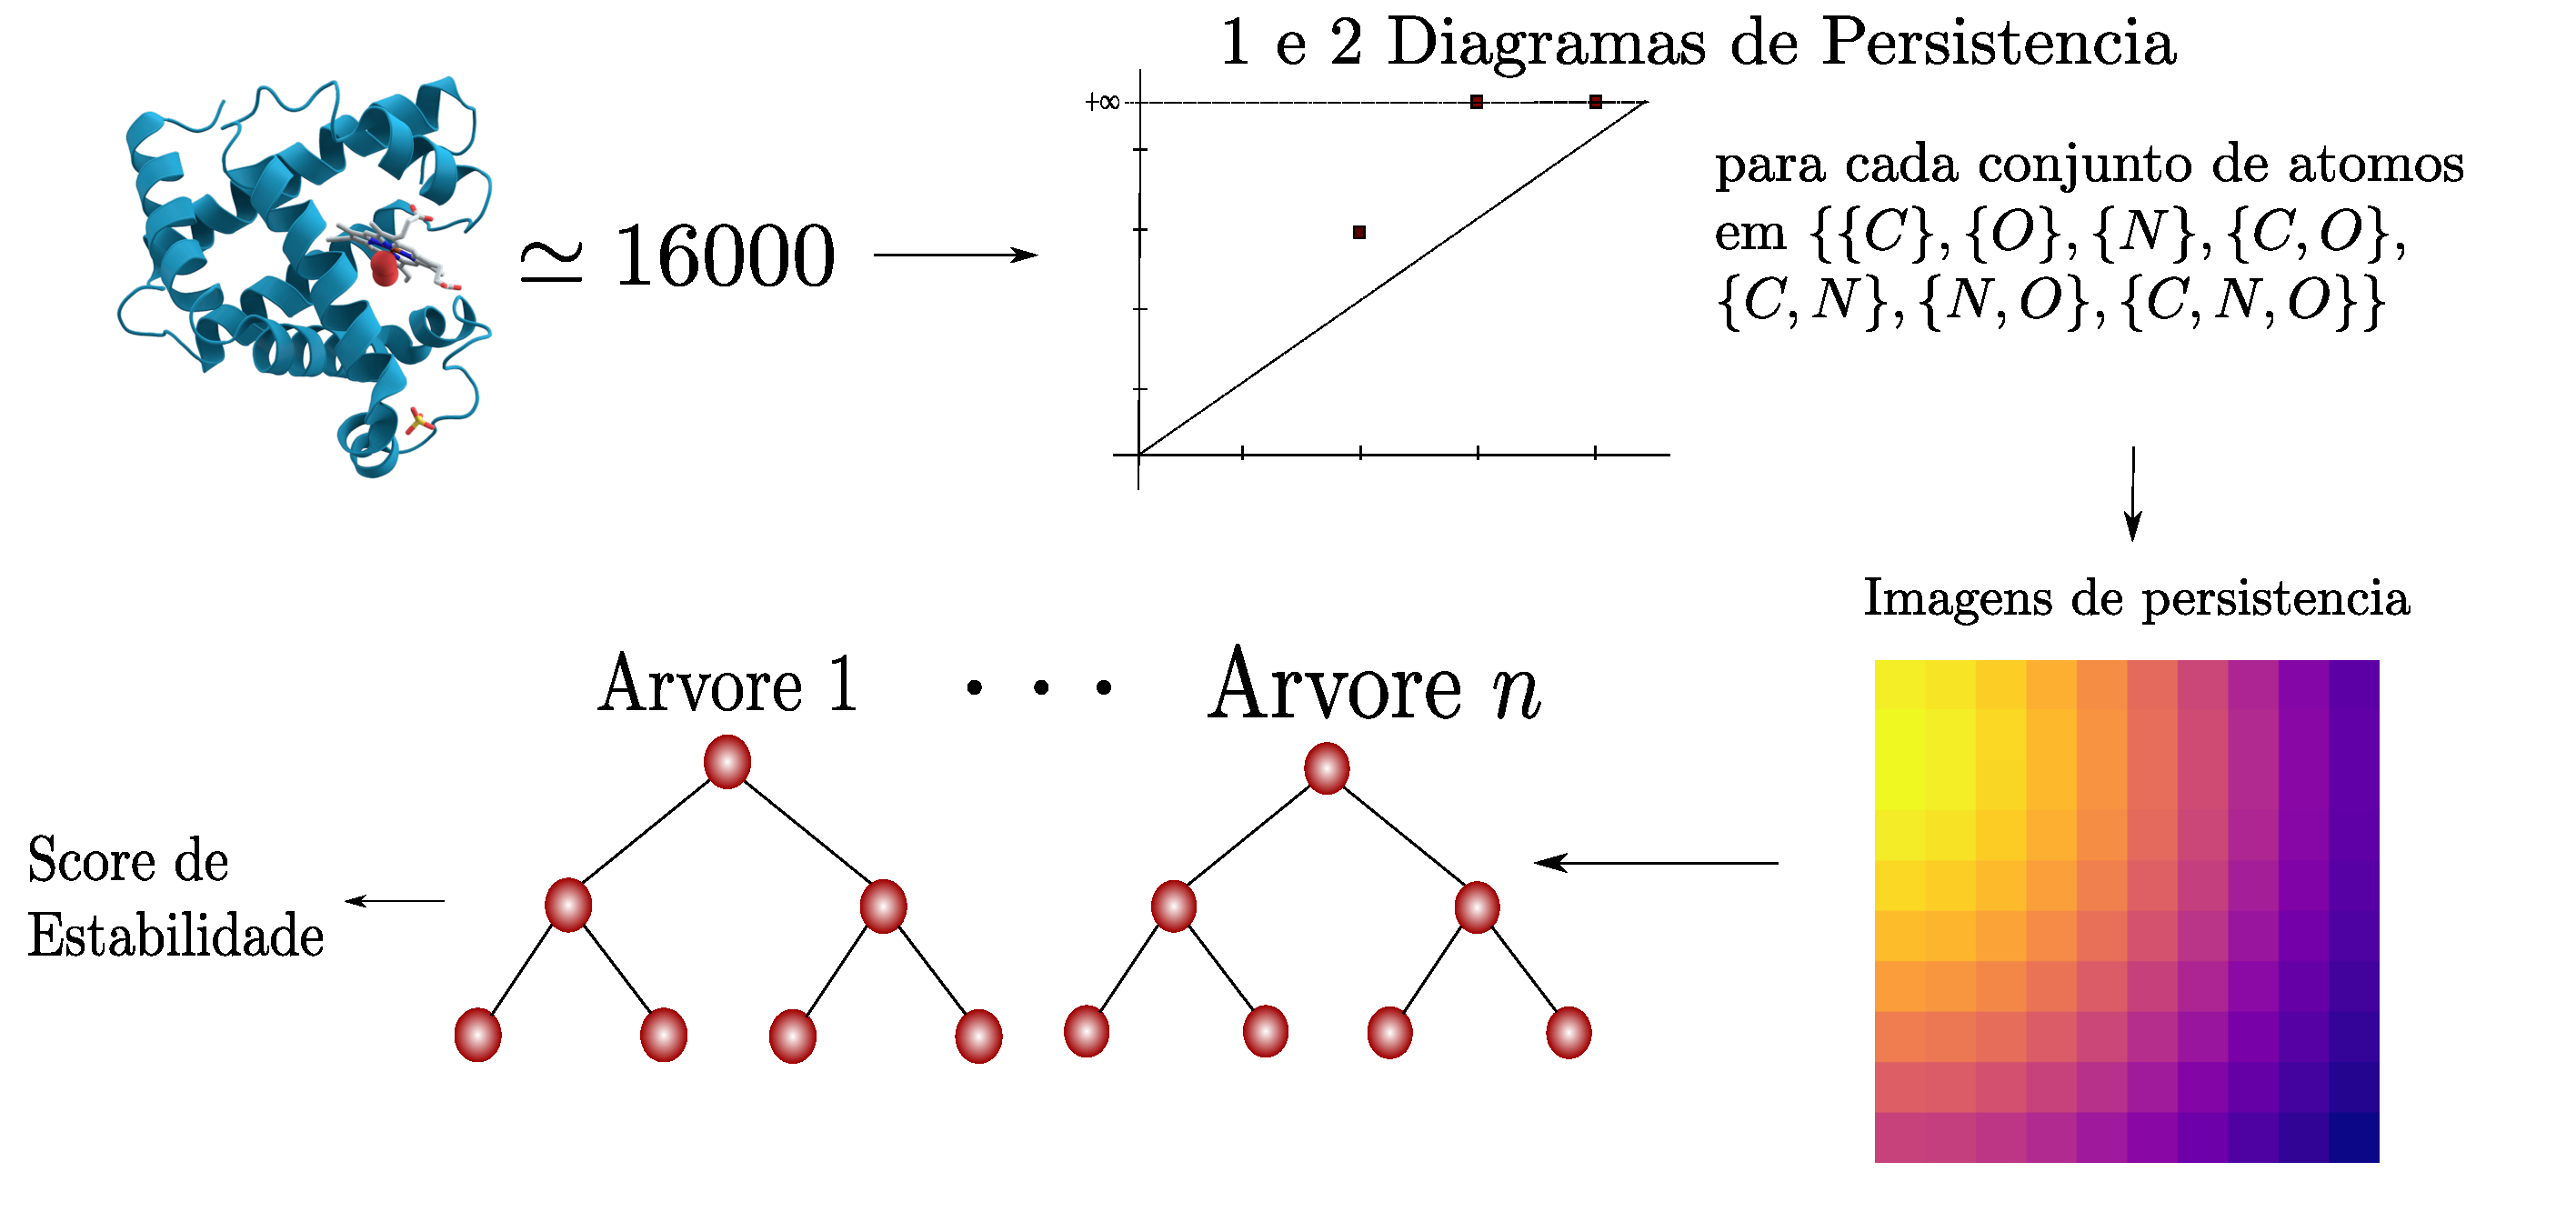
\includegraphics[width=0.99\textwidth]{images/proteinpipeline.pdf}
    \caption{Pipeline da metodologia utilizada para a predição do score de estabilidade.} 
    \label{fig:proteinpipeline}
    \fautor 
\end{figure}

\subsection{Resultados e análises} 
\subsubsection{Primeiro método}
O primeiro método consiste em utilizar as propriedades da proteínas e as imagens de 
persistência para prever o score de estabilidade. Temos 4 tabelas para cada uma das 
variâncias. 

\begin{table}[htpb!]
    \centering
    \caption{Resultados para variância igual a $0,1$.}
    \label{tab:var01}
    \begin{tabular}{@{}ccccc@{}}
    \toprule
    Modelo                 & MSE    & RMSE   & Erro Percentual (\%) & $R^2$  \\ \midrule
    GBoost                 & 0,1831 & 0,4278 & 11,61                & 0,5529 \\
    Regressão Linear       & 0,2025 & 0,4500 & 12,21                & 0,5054 \\
    Regressão lin. c/ Reg. & 0,2084 & 0,4565 & 12,39                & 0,4910 \\
    Árvore de decisão I    & 0,1771 & 0,4208 & 11,42                & 0,5674 \\
    Árvore de decisão II   & 0,1780 & 0,4219 & 11,45                & 0,5653 \\ \bottomrule
    \end{tabular}
\end{table}
\begin{table}[htpb!]
    \centering
    \caption{Resultados para variância igual a $0,3$.}
    \label{tab:var03}
    \begin{tabular}{@{}ccccc@{}}
    \toprule
    Modelo                 & MSE    & RMSE   & Erro Percentual (\%) & $R^2$  \\ \midrule
    GBoost                 & 0,1832 & 0,4281 & 11,62                & 0.5525 \\
    Regressão Linear       & 23,6637 & 4,8645 & 132,01                & -56.7950 \\
    Regressão lin. c/ Reg. & 0,2075 & 0,4555 & 12,36                & 0,4932 \\
    Árvore de decisão I    & 0,1772 & 0,4209 & 11,42                & 0,5672 \\
    Árvore de decisão II   & 0,1785 & 0,4225 & 11,46                & 0,5641 \\ \bottomrule
    \end{tabular}
\end{table}
\begin{table}[htpb!]
    \centering
    \caption{Resultados para variância igual a $0,5$.}
    \label{tab:var05}
    \begin{tabular}{@{}ccccc@{}}
    \toprule
    Modelo                 & MSE    & RMSE   & Erro Percentual (\%) & $R^2$  \\ \midrule
    GBoost                 & 0,1829 & 0,4277 & 11,61 & 0,5533 \\
    Regressão Linear       & 0,2032 & 0,4508 & 12,23 & 0,5036 \\
    Regressão lin. c/ Reg. & 0,2068 & 0,4548 & 12,34 & 0,4949 \\
    Árvore de decisão I    & 0,1781 & 0,4220 & 11,45 & 0,5650 \\
    Árvore de decisão II   & 0,1783 & 0,4222 & 11,46 & 0,5646 \\
    \bottomrule
    \end{tabular}
\end{table}
\begin{table}[htpb!]
    \centering
    \caption{Resultados para variância igual a $0,7$.}
    \label{tab:var07}
    \begin{tabular}{@{}ccccc@{}}
    \toprule
    Modelo                 & MSE    & RMSE   & Erro Percentual (\%) & $R^2$  \\ \midrule
    GBoost                 & 0,1828 & 0,4275 & 11,60 & 0,5536 \\
    Regressão Linear       & 0,2009 & 0,4482 & 12,16 & 0,5093 \\
    Regressão lin. c/ Reg. & 0,2069 & 0,4549 & 12,34 & 0,4947 \\
    Árvore de decisão I    & 0,1779 & 0,4218 & 11,45 & 0,5655 \\
    Árvore de decisão II   & 0,1790 & 0,4230 & 11.48 & 0,5629 \\
    \bottomrule
    \end{tabular}
\end{table}

Esperavamos obter resultados melhores quando combinassemos ambos os conjuntos de dados em um só, mas
os resultados ficaram bem similares. Acreditamos que o resultado continua similar pois as propriedades
dadas pelas imagens da persistência possuem uma correlação com propriedades já conhecidas de proteínas, 
sendo assim a adição de novas propriedades não melhora o algoritmo. 

Os parâmetros para os algoritmos são os seguintes:
\begin{itemize}
    \item GBoost: n\_estimators $\in [100,300,500,700]$, min\_samples\_split $\in [2,5,10,15]$;
    \item Árv. Dec. I: n\_estimators $=689$, max\_features $=0.2$, max\_depth $=86$;
    \item Árv. Dec. II: n\_estimators $=500$, max\_depth $=100$, max\_features $=0.3$;
    \item Regressão Lin. c/ Reg: valor de alfa em $[0.005, 5000]$ (de $10$ em $10$) escolhido com 
     cross validation de 5 folds. 
\end{itemize}

\subsubsection{Segundo método}

Para o segundo método, utilizamos apenas as imagens de persistência para o treinamento. Obtivemos
um resultado similar ao dos modelos treinados com as propriedades das proteínas apenas. Os resultados
podem ser vistos nas tabelas a seguir. Note também como os resultados melhoram quando aumentamos
a variância utilizadada para as imagens de persistência. 

\begin{table}[htpb!]
\centering
\caption{Resultados dos modelos treinados utilizando apenas as imagens de persistência com variância
$0.1$}
\label{tab:pionly01}
\begin{tabular}{@{}ccccc@{}}
\toprule
Modelo                 & MSE    & RMSE   & Erro Percentual (\%) & $R^2$  \\ \midrule
Regressão Linear       & 0,2734 & 0,5229 & 14,19                & 0,3322 \\
GBoost                 & 0,2435 & 0,4935 & 13,39                & 0,4053 \\
Árvore de Decisão I    & 0,2490 & 0,4990 & 13,54                & 0,3917 \\
Árvore de Decisão II   & 0,2485 & 0,4985 & 13,53                & 0,3931 \\
Regressão Lin. c/ Reg. & 0,2723 & 0,5218 & 14,16                & 0,3350 \\
GBoost Ótimo           & 0,2450 & 0,4950 & 13,43                & 0,4017 \\ \bottomrule
\end{tabular}
\end{table}
\begin{table}[htpb!]
\centering
\caption{Resultados dos modelos treinados utilizando apenas as imagens de persistência com variância
$0.3$}
\label{tab:pionly03}
\begin{tabular}{@{}ccccc@{}}
\toprule
Modelo                 & MSE      & RMSE    & Erro Percentual (\%) & $R^2$      \\ \midrule
Regressão Linear       & 438,3102 & 20,9359 & 568,14               & -1069,5076 \\
GBoost                 & 0,2364   & 0,4863  & 13,20                & 0,4225     \\
Árvore de Decisão I    & 0,2417   & 0,4917  & 13,34                & 0,4096     \\
Árvore de Decisão II   & 0,2419   & 0,4919  & 13,35                & 0,4091     \\
Regressão Lin. c/ Reg. & 0,2649   & 0,5146  & 13,97                & 0,3531     \\
GBoost Ótimo           & 0,2305   & 0,4801  & 13,03                & 0,4371     \\
\bottomrule
\end{tabular}
\end{table}
\begin{table}[htpb!]
\centering
\caption{Resultados dos modelos treinados utilizando apenas as imagens de persistência com variância
$0.5$}
\label{tab:pionly05}
\begin{tabular}{@{}ccccc@{}}
\toprule
Modelo                 & MSE    & RMSE   & Erro Percentual (\%) & $R^2$  \\ \midrule
Regressão Linear       & 0,2639 & 0,5137 & 13,94 & 0,3555 \\
GBoost                 & 0,2327 & 0,4824 & 13,09 & 0,4316 \\
Árvore de Decisão I    & 0,2409 & 0,4908 & 13,32 & 0,4117 \\
Árvore de Decisão II   & 0,2403 & 0,4902 & 13,30 & 0,4130 \\
Regressão Lin. c/ Reg. & 0,2594 & 0,5093 & 13,82 & 0,3665 \\
GBoost Ótimo           & 0,2328 & 0,4825 & 13,09 & 0,4314 \\ \bottomrule
\end{tabular}
\end{table}
\begin{table}[htpb!]
\centering
\caption{Resultados dos modelos treinados utilizando apenas as imagens de persistência com variância
$0.7$}
\label{tab:pionly07}
\begin{tabular}{@{}ccccc@{}}
\toprule
Modelo                 & MSE    & RMSE   & Erro Percentual (\%) & $R^2$  \\ \midrule
Regressão Linear       & 0,2546 & 0,5046 & 13,69 & 0,3781 \\
GBoost                 & 0,2342 & 0,4839 & 13,13 & 0,4281 \\
Árvore de Decisão I    & 0,2379 & 0,4877 & 13,24 & 0,4190 \\
Árvore de Decisão II   & 0,2376 & 0,4874 & 13,23 & 0,4197 \\
Regressão Lin. c/ Reg. & 0,2535 & 0,5035 & 13,66 & 0,3809 \\
GBoost Ótimo           & 0,2276 & 0,4770 & 12,95 & 0,4442 \\ \bottomrule
\end{tabular}
\end{table}
Observamos que o melhor resultado é para o GBoost ótimo com variância $0,7$. Como o GBoost
é um método de árvores de decisão, ele nos dá a importância de cada uma das propriedades
dos vetores. Vamos fazer uma análise dessas propriedades. 

Primeiro, precisamos selecionar um número significativo de propriedades, já que algumas são
mais importantes que as outras. Cada propriedade tem um número associado a ela, dado pelo
algoritmo GBoost. A soma de todas esses valores da 1. Na Figura~\ref{fig:knee_plot} temos 
o logaritmo do valor da soma acumulada da propriedade com maior valor de importância até a última. 
\begin{figure}
    \centering
    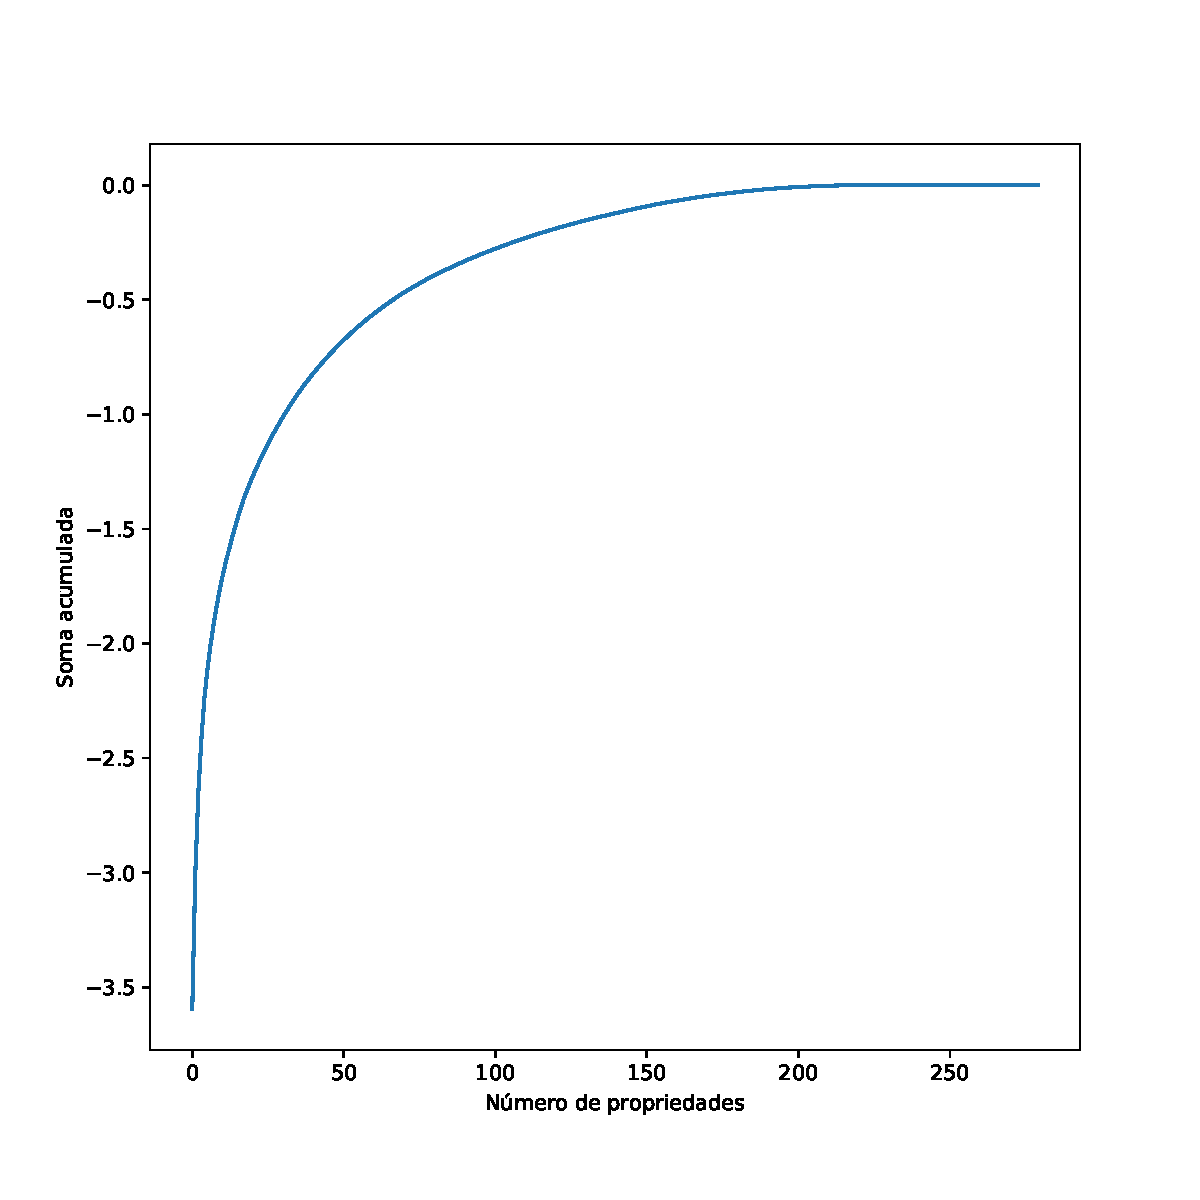
\includegraphics[width=0.7\textwidth]{images/plt_ankle.pdf}
    \caption{Logaritmo da soma acumulada em relação à importância das propriedades dado pelo algoritmo
    GBoost.}
    \label{fig:knee_plot}
    \fautor
\end{figure}
Note como o plot dobra ao redor do número 50. Isso significa que as 50 primeiras propriedades são
as mais importantes, já contribuem mais para a soma acumulada. Pela construção das imagens
de persistência, temos que cada propriedade está relacionada com uma certa região da vetorização
do diagrama. Portanto, podemos localizar as regiões dos diagramas de persistência que 
aparecem nas propriedades. Dentre as 50 propriedades mais importantes, temos que a maioria
vem de pontos dos diagramas de dimensão 1 e correspondem a pontos com nascimentos logo
no início da filtração e com persistência baixa, como pode ser visto nas Figuras~\ref{fig:count_pd}
e~\ref{fig:count_pd2}
\begin{figure}[htpb!]
    \begin{minipage}{0.5\textwidth}
        \centering
        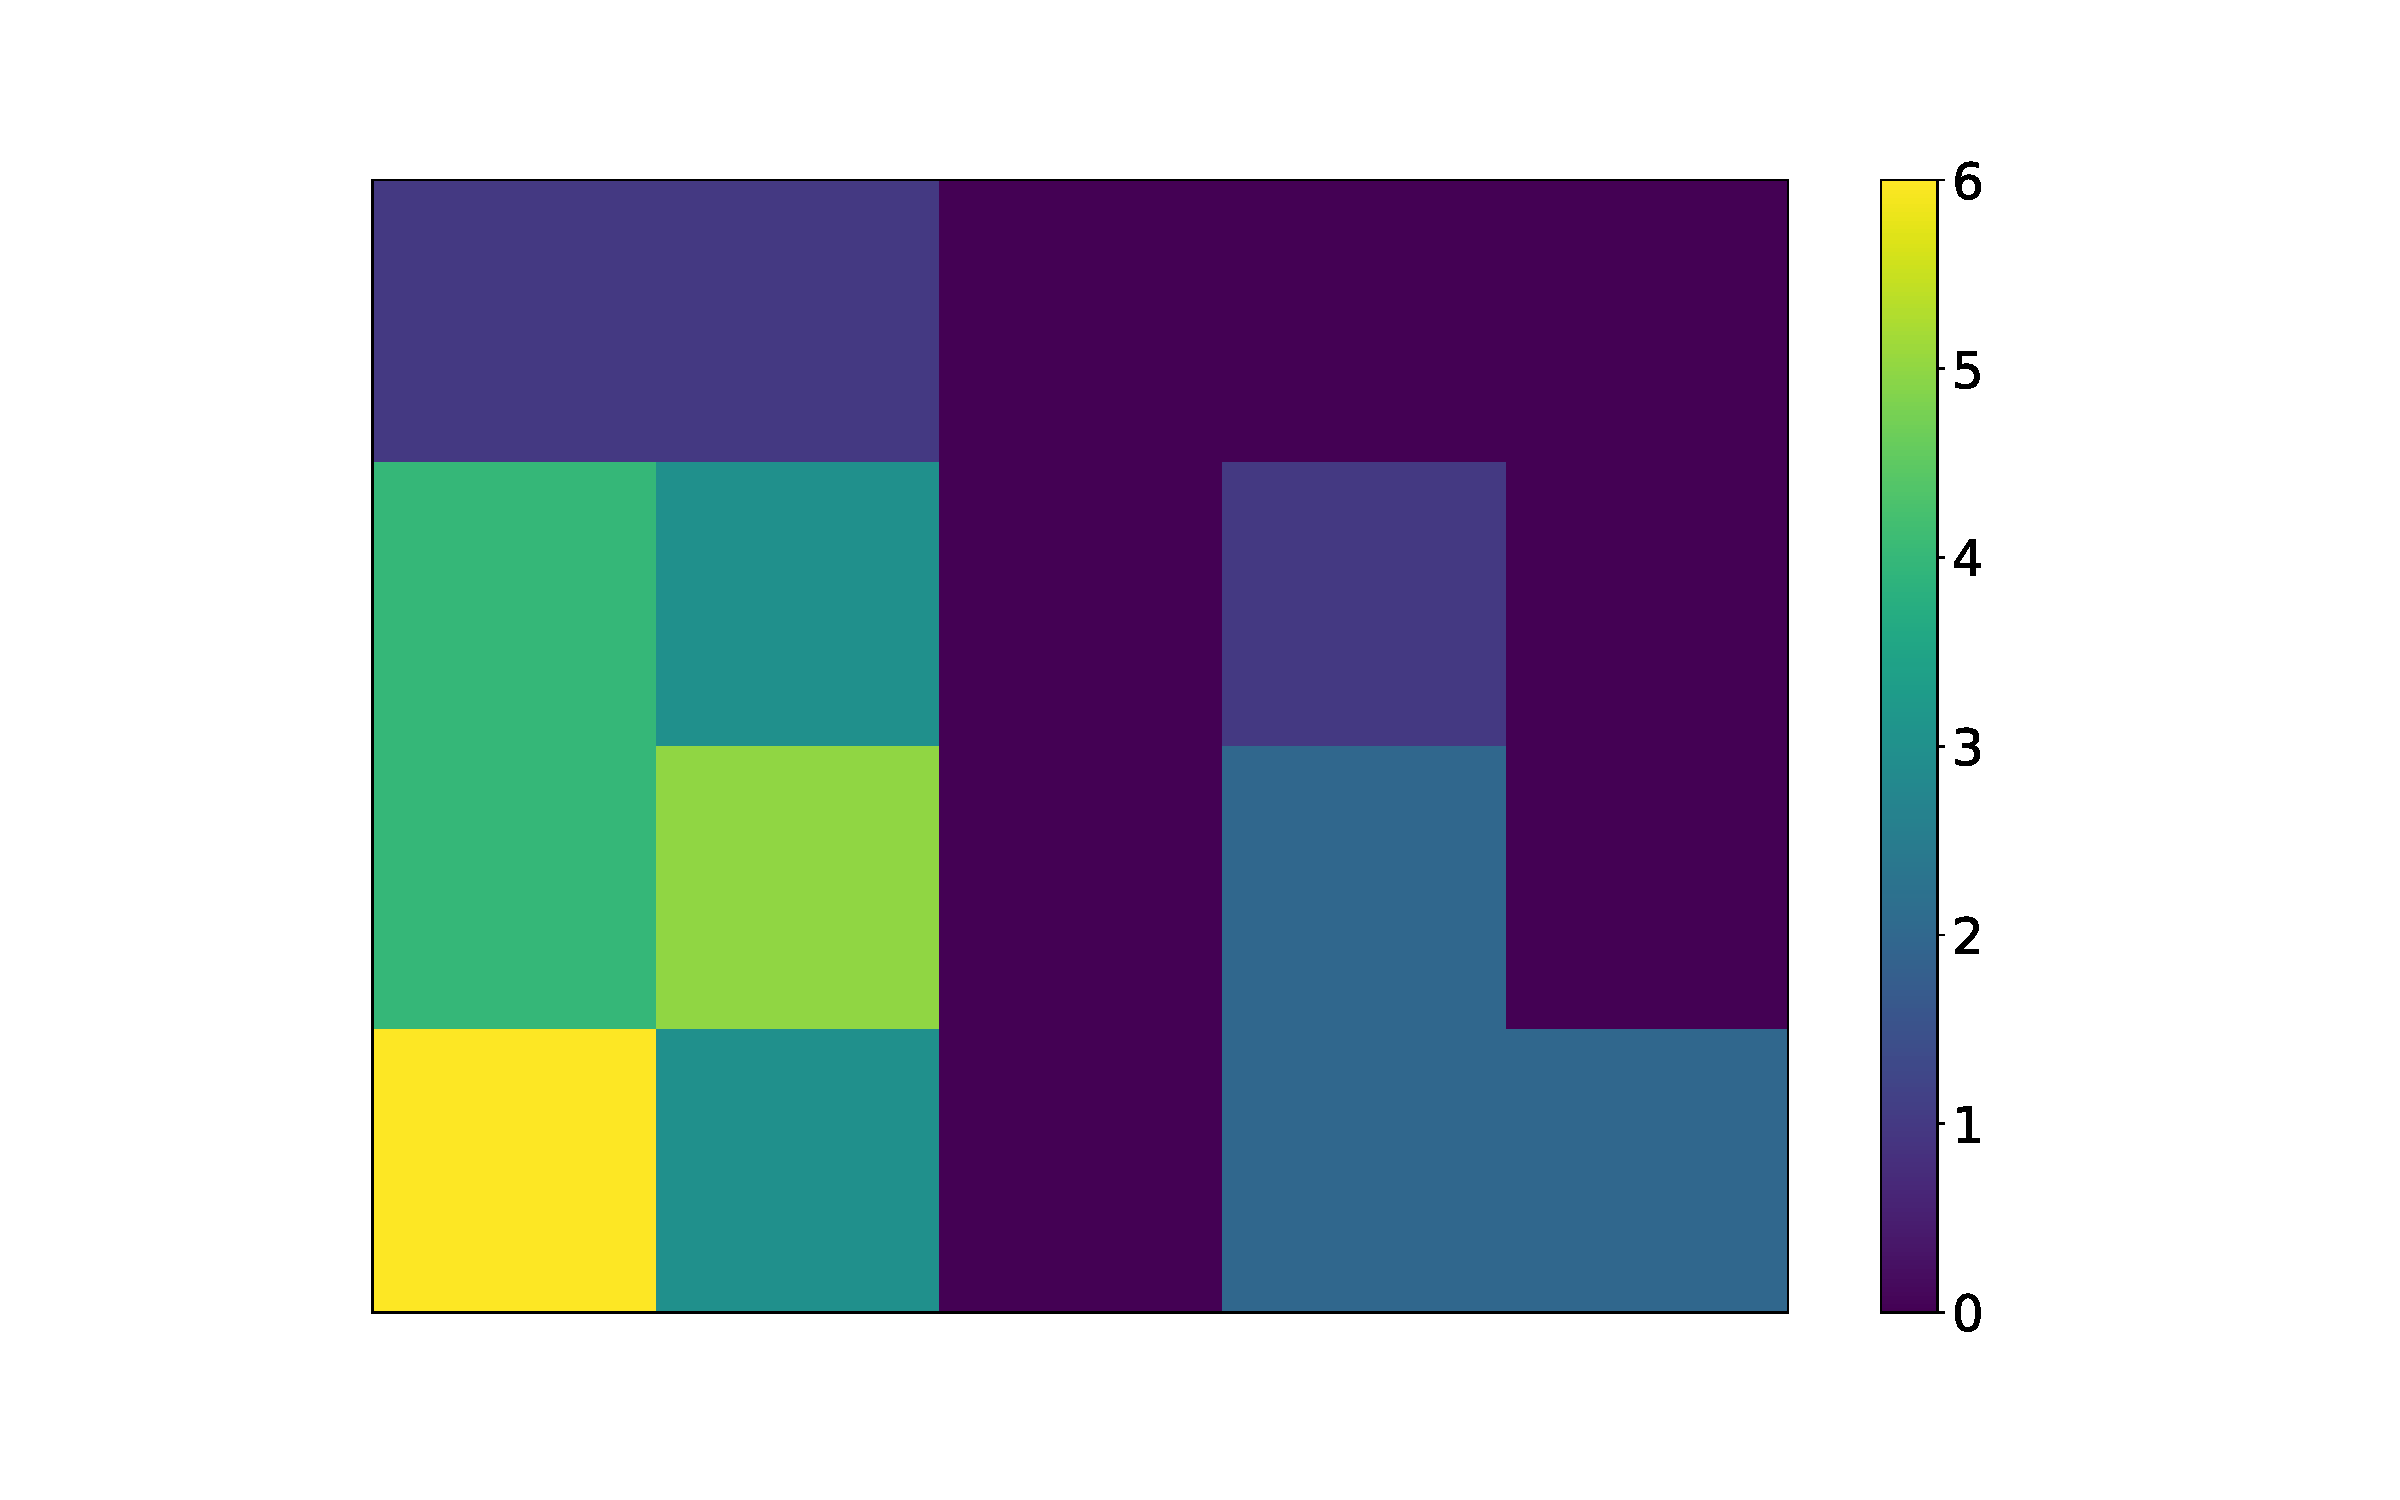
\includegraphics[width=1.1\textwidth]{images/heatmap_1.pdf}
        \caption{Heatmap das regiões dos diagramas de persistência de dimensão 1 que aparecem
        nas primeiras 50 propriedades. Eixo x representa nascimento, enquanto que o eixo y 
        representa a persistência.}
        \label{fig:count_pd}
        \fautor
    \end{minipage}
    \begin{minipage}{0.5\textwidth}
        \centering
        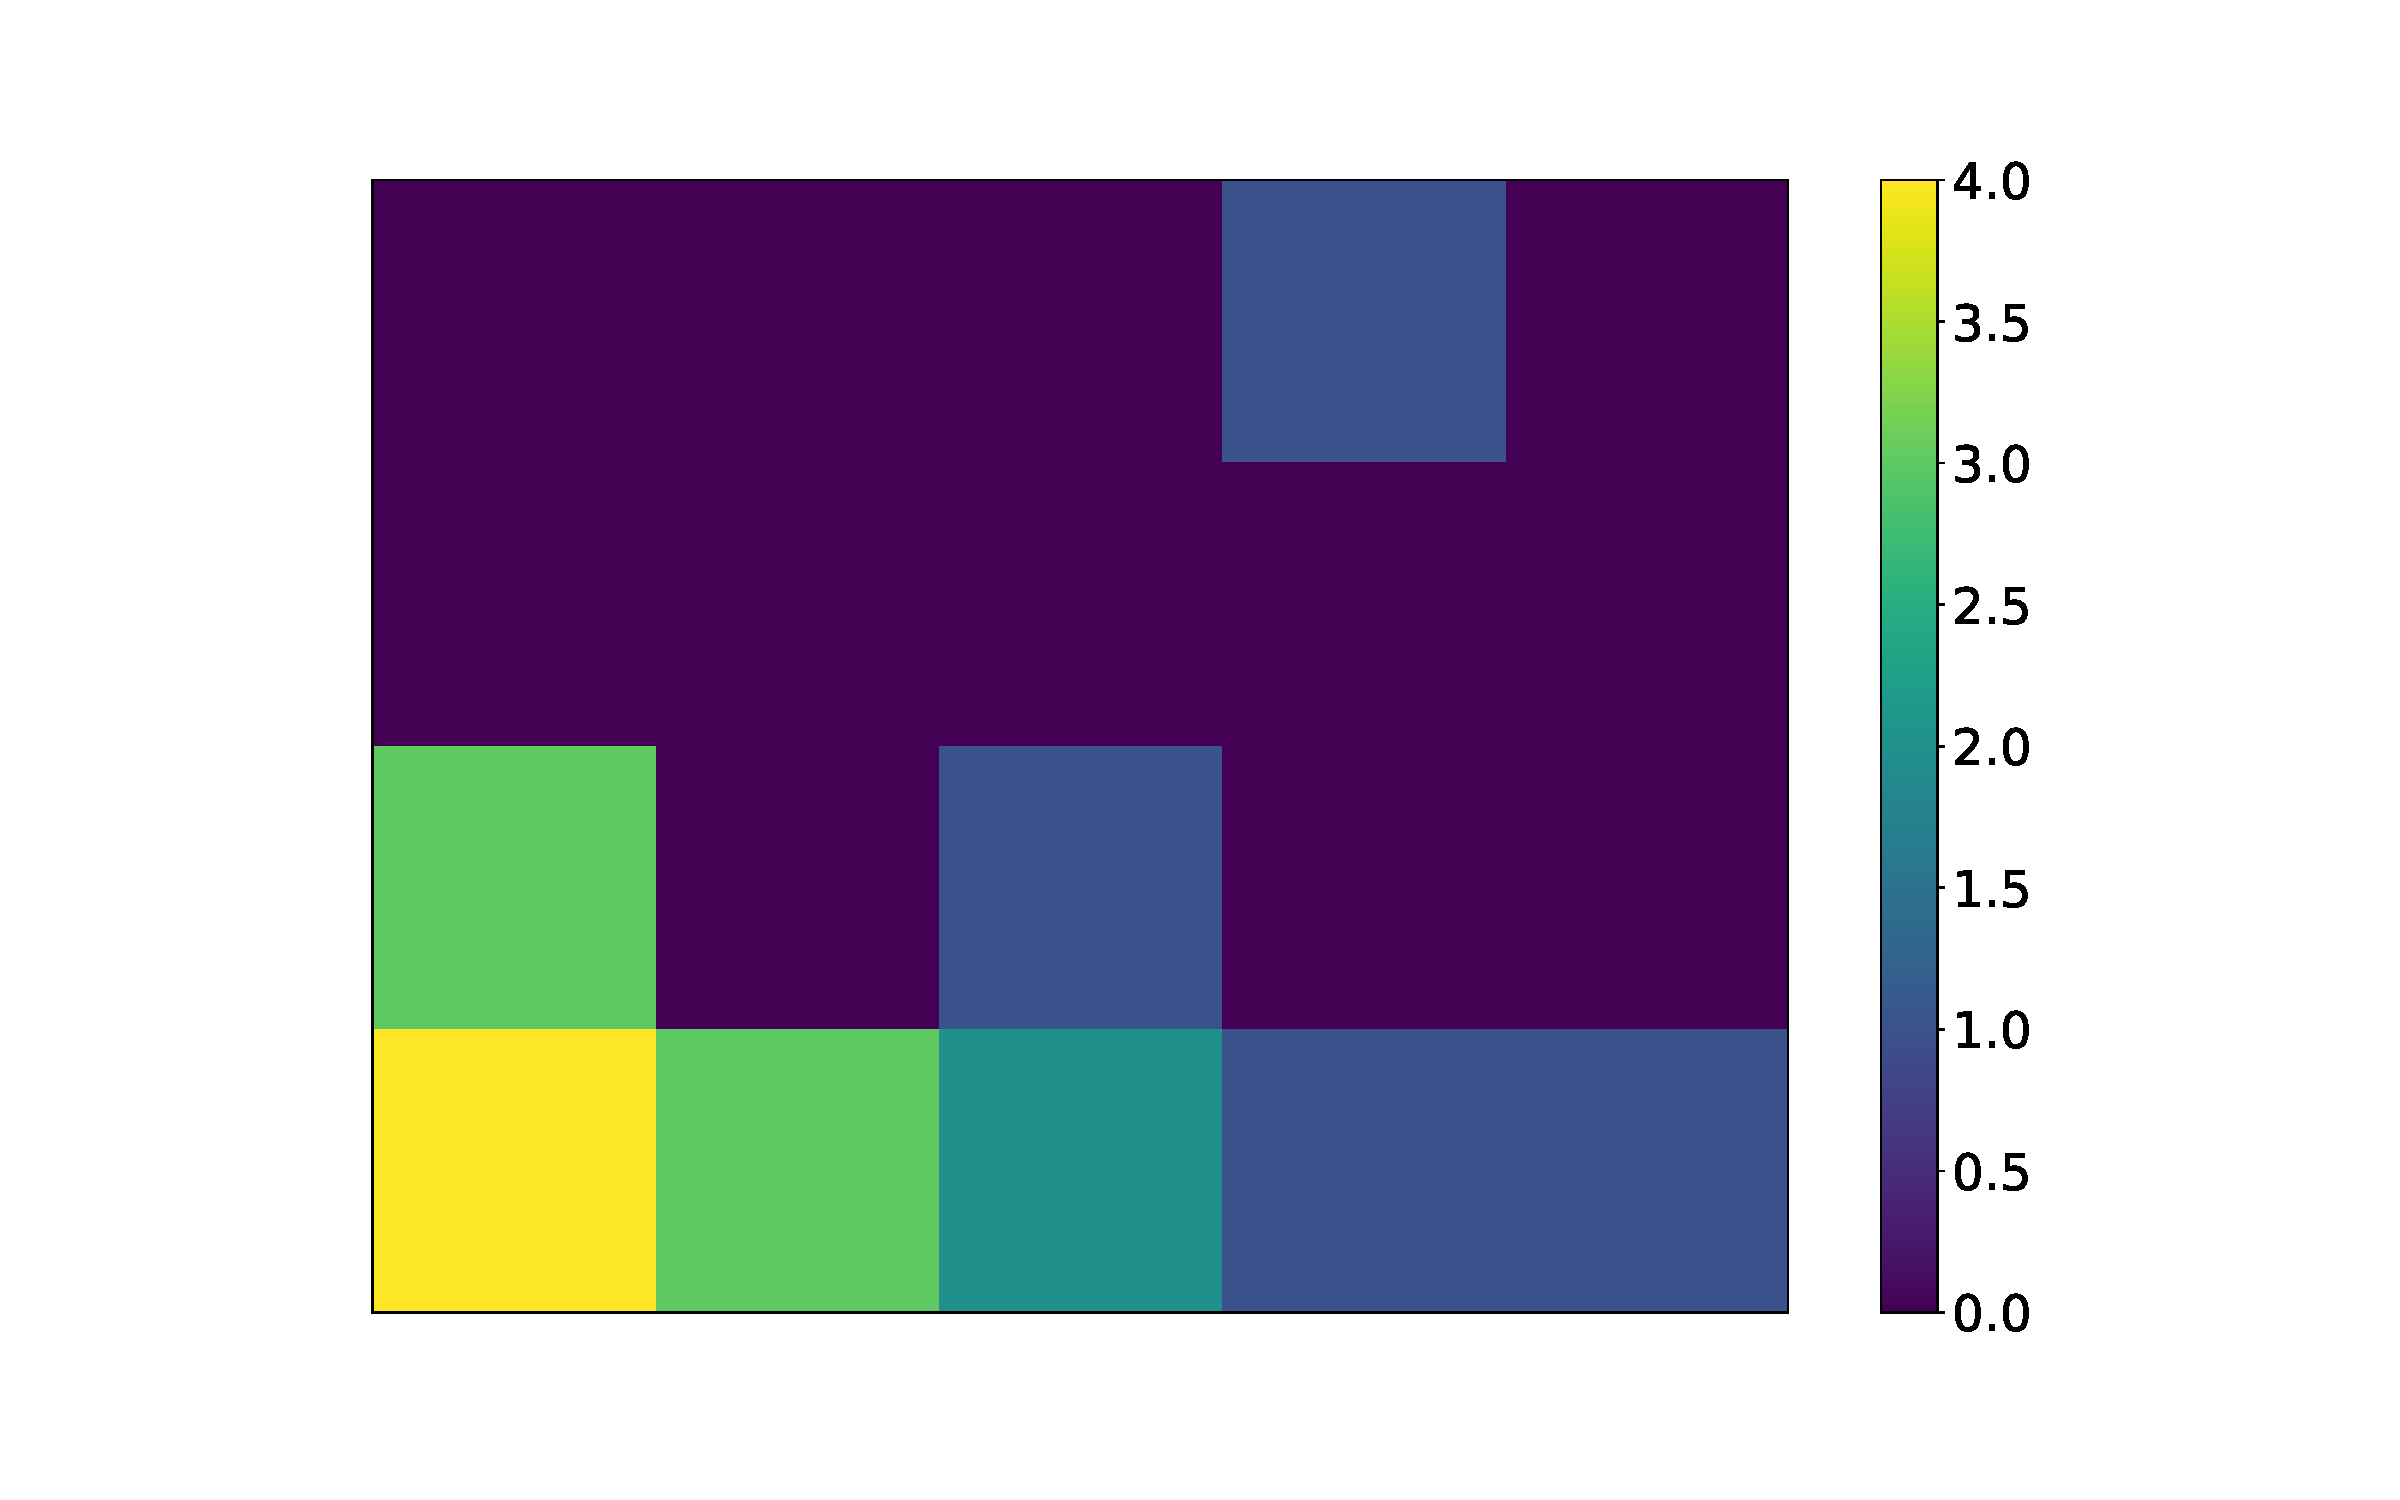
\includegraphics[width=1.1\textwidth]{images/heatmap_2.pdf}
        \caption{Heatmap das regiões dos diagramas de persistência de dimensão 2 que aparecem
        nas primeiras 50 propriedades. Eixo x representa nascimento, enquanto que o eixo y 
        representa a persistência.}
        \label{fig:count_pd2}
        \fautor
    \end{minipage}
\end{figure}
 
Dentre as propriedades mais importantes podemos analisar também a que conjunto de átomos elas estão 
associadas quando os diagramas de persistência foram calculados. Observamos na Figura~\ref{fig:plt_dim}
que os átomos associados aos ciclos que mais aparecem são os encontrados nos diagramas de persistência
calculados utilizando apenas carbono e nitrogênio. Os autores de~\cite{Cang2018} afirmam que 
ciclos associados a esses átomos representam propriedades hidrofóbicas e hidrofílicas, 
características que influenciam diretamente na estabilidade da proteína.  

\begin{figure}[htpb!]
    \centering
    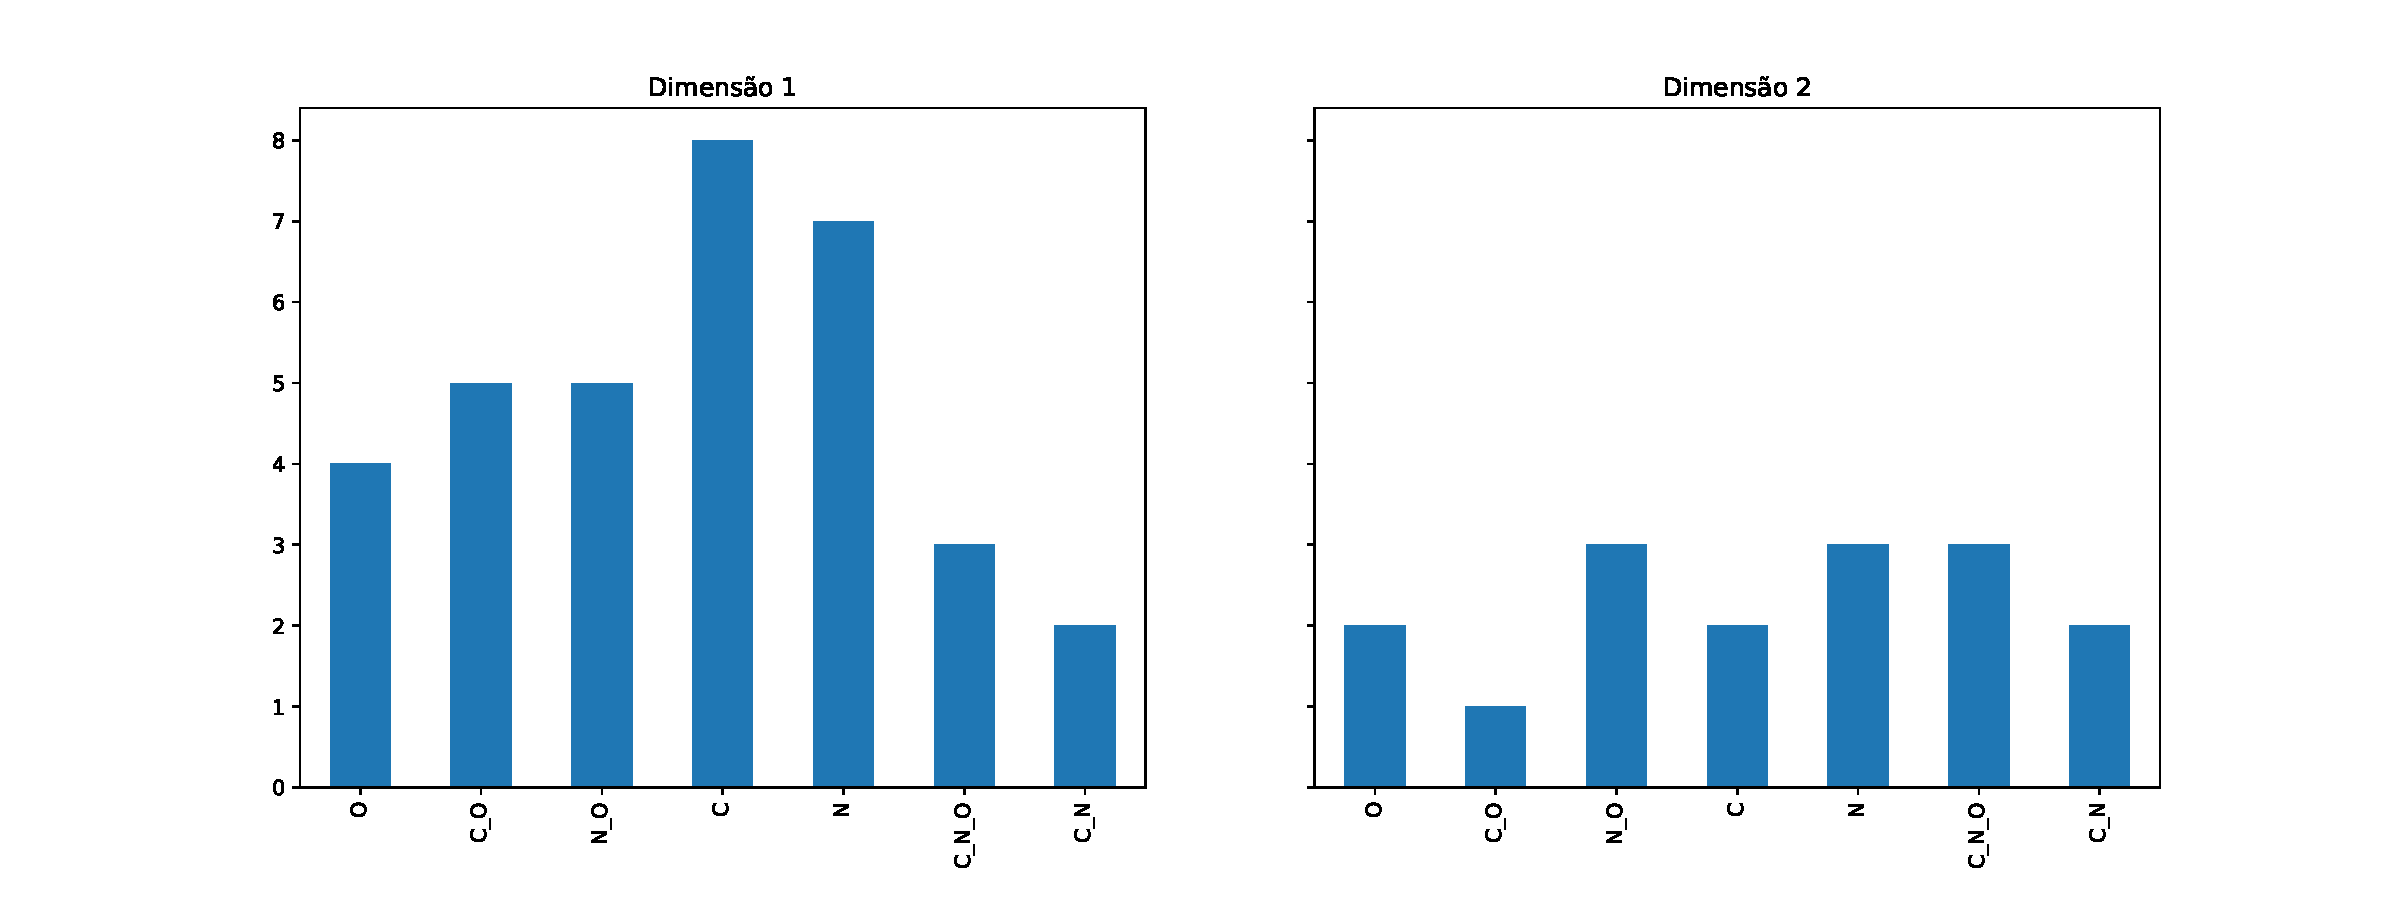
\includegraphics[width=0.99\textwidth]{images/plt_dim.pdf}
    \caption{Número de ciclos associados para as top 50 propriedades e seus respectivos 
        diagramas de persistência.}
    \label{fig:plt_dim}
    \fautor
\end{figure}

\section{Analisando a energia total - Proteínas II}\label{sec:predrmsd}

Em \cite{Rubenstein2018} eles analisam a eficácia do \textit{Rosetta} e \textit{Amber}, dois softwares
para modelagem de macromoléculas. Dado uma proteína obtida do Protein Data Bank (PDB), por exemplo a proteína
de ID 1T2I, eles geraram novas moléculas usando amostragem ab-inition com viés e sem viés seguido por
uma amostragem paralela loophash. Após isso, essas amostras foram sujeitas à minimização no
backbone (átomos C-$\alpha$) e cadeias laterais (grupo-R) usando o protocolo talaris2014 e o minimzador
LBFGS. Então com os átomos C-$\alpha$ apenas, o RMSD foi calculado para todos as decoys (moléculas
geradas pelo software).

\begin{figure}[!htbp]
    \centering
    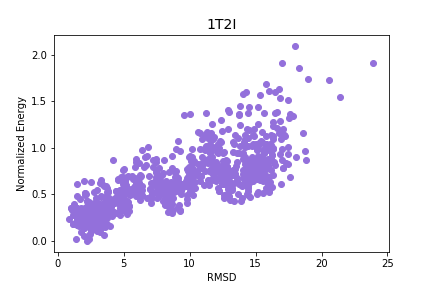
\includegraphics[width=0.7\textwidth]{images/relatorio/1t2i_tunnel.png}
    \caption{Panorama de energia para decoys modeladas em relação à proteína 1T2I.}
    \label{fig:1t2iland}
    \fautor
\end{figure}

Para cada decoy existe um score de energia associado, que é a função score minimizada pelo \textit{Rosetta}.
Com esse valor podemos plotar o panorama de energia para cada proteína, como na Figura~\ref{fig:1t2iland}.
O formato ideal seria o de um túnel, já que RMSD baixo corresponderia a uma energia normalizada baixa idealmente.

O score de energia dado por \textit{Rosetta} é normlizado usando a seguinte fórmula
\begin{equation}
    E_{i(norm)} = \frac{E_i - E_{\min}}{E_{95th} - E_{5th}},
\end{equation}
em que $E_{95th}$ é o $95$-ésimo percentil e $E_{5th}$ é o quinto percentil.

\subsection{Análise de falso mínimos}
Dados as moléculas geradas pelo software, podemos ranquear cada decoy de acordo com sua energia normalizada
e RMSD. Ranqueamos o conjunto de decoys da menor para a maior energia, por exemplo uma molécula com energia
de 0.3 está acima de outra com energia 0.5 no ranking. Na Tabela~\ref{tab:protrank} temos o top 5 decoys
das proteínas geradas a partir da 1T2I.

\begin{table}[!htbp]
    \centering
    \caption{Rank mostrando as top 5 decoys em relação a 1T2I.}
    \label{tab:protrank}
    \begin{tabular}{@{}ccc@{}}
        \toprule
        Rank & Energia normalizada & RMSD  \\
        \midrule
        1    & 0.000             & 2.233 \\
        2    & 0.023             & 1.37  \\
        3    & 0.025             & 2.395 \\
        4    & 0.057             & 2.004 \\
        5    & 0.061             & 2.356 \\
        \bottomrule
    \end{tabular}
\end{table}

Como mencionado anteriormente, \textit{Rosetta} tenta minimizar uma função score de energia de forma
que energia baixa corresponde a um valor baixo do RMSD. Dizemos que uma decoy é um falso mínimo
se está no top 10 moléculas do ranking de acordo com a definição acima e também possui um RMSD maior
do que $5$.

\subsubsection{VAE e ciclos ótimos}

Para analisar os falsos mínimos, utilizamos homologia persistente \cite{Edelsbrunner2002} para extrair
informações biológicas, como hidrofobicidade, juntamente com outras ferramentas topológicas \cite{Cang2017}.

Para cada ponto no diagrama de persistência existe um ciclo, um representante para sua respectiva classe
de homologia, que possui propriedades geométricas dos dados. Apesar disso, os ciclos não possuem o
verdadeiro tamanho do correspondente buraco $n$-dimensional, com respeito ao número de arestas. Portanto,
o problema de encontrar o ciclo ótimo em relação ao número de arestas é muito interessante, já que assim
podemos representar as propriedades topológicas de maneira muito mais fiel \cite{Escolar2015}.

Por um lado ciclos ótimos codificam muita informação, por outro lado é muitas vezes difícil analisa-los
de forma coesa. Portanto, nós propomos um método similar a \cite{Obayashi2018}. Primeiro vetorizamos
os diagramas de persistência utilizando imagens de persistência \cite{Adams2017} e após isso treinamos
um autoencoder variacional básico \cite{kingma2013} para extrair as regiões mais importantes
da imagem de persistência. Então realizamos uma análise inversa, em que para
cada região da imagem, existem pontos associados no diagrama de persistência e dessa forma seus
respectivos ciclos. Então, para cada conjunto de ciclos, somamos todos os átomos correspondentes de
cada ciclo, por xemplo, soma de todos os átomos de carbono de todos os ciclos. 

Nas próximas subseções
mostramos os resultados e parâmetros utilizados para gerar os diagramas de persistência, imagens
de persistência e hiperparâmetros para o treinamento do VAE.

\subsubsection{Resultados}

Selecionamos as proteínas de ID 2QY7 e 1T2I para análise. A primeira contém vários falsos mínimos,
enquanto a última não possui falso mínimo.

Para a proteína 2QY7 calculamos os diagramas de persistência para os top 100 decoys e plotamos a
soma na Figura~\ref{fig:cyc2qy7}.

\begin{figure}[!htbp]
    \centering
    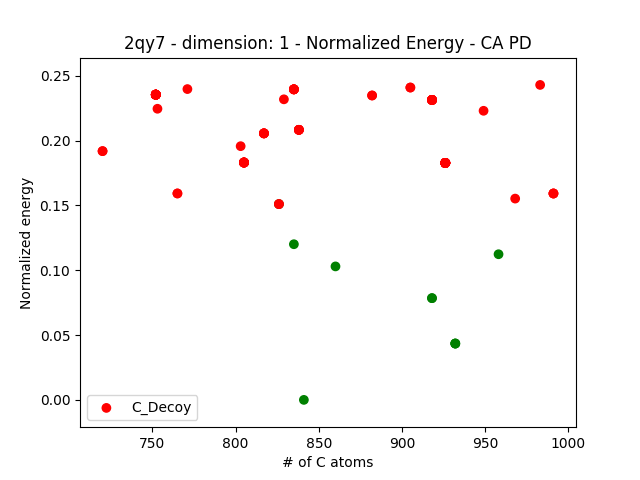
\includegraphics[width=0.7\textwidth]{images/relatorio/cyc2qy7.png}
    \caption{Soma dos átomos de carbono que compõem os ciclos do
            $1^\circ$ diagrama de persistência das decoys da 2QY7.}
    \label{fig:cyc2qy7}
    \fautor
\end{figure}

Para cada decoy foi calculado dois diagramas de persistência, um para a dimensão 1 e outro para a dimensão 2.
Em cada uma das dimensões usamos duas nuvens de pontos, a primeiro composta apenas pelos átomos C-$\alpha$
das moléculas e a outra composta apenas pelos átomos de nitrogênio e oxigênio.

Note que quando usamos apenas os átomos de carbono, a maioria dos falsos mínimos ficam agrupados em um intervalo
pequeno, como pode ser visto na Figura~\ref{fig:cyc2qy7}, e por outro lado com a outra nuvem de pontos os valores
ficaram espalhados, indicando que para esta proteína é melhor usar os átomos C-$\alpha$ para análise de falsos
mínimos.

Já para a proteína 1T2I um fenômeno similar acontece, como pode ser visto na Figura~\ref{fig:nocyc}. As top decoys
ficam em um intervalo menor, enquanto outras moléculas estão espalhadas pelo intervalo.
\begin{figure}[!htbp]
    \centering
    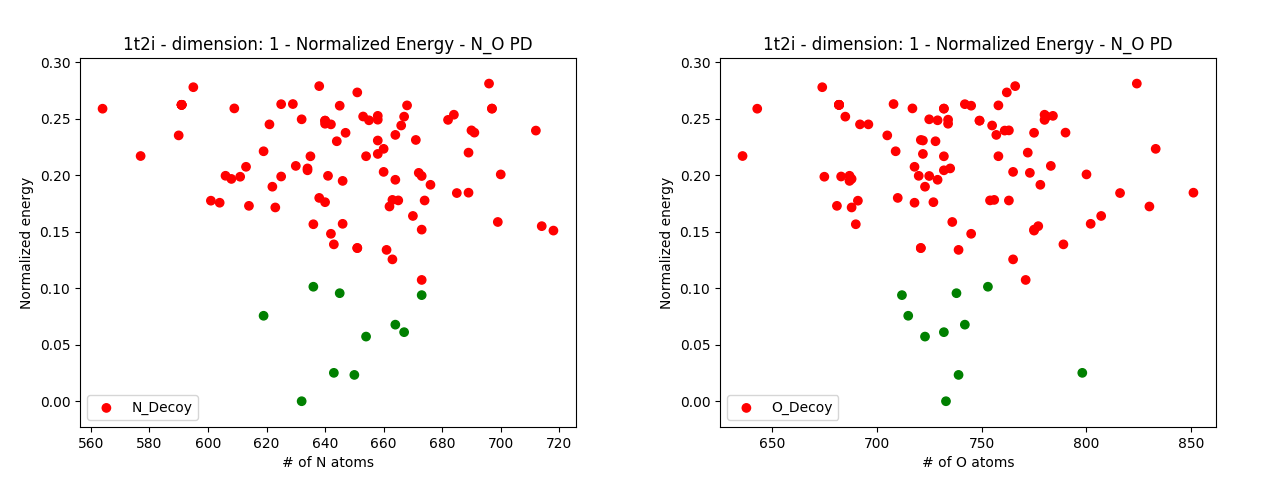
\includegraphics[width=0.99\textwidth]{images/relatorio/NOcyc.png}
    \caption{Soma dos átomos de nitrogênio (esquerda) e oxigênio (direita) que compõe os cyclos do 
    $1^\circ$ diagrama de persistência das decoys da proteína 1T2I.}    
    \label{fig:nocyc}
    \fautor
\end{figure}

É importante notar que os ciclos da proteína com um panorâma de energia bom (1T2I) foram melhor caracterizados
pelos átomos de nitrogênio e oxigênio, enquanto que para a outra proteína, os átomos C-$\alpha$ caracterizaram melhor.

\subsubsection{Parâmetros}

Calcumos os primeiro e segundo diagramas de persistência usando a filtração alpha, onde o raio de cada átomo
era o raio de Van der Waals. Para os ciclos ótimos o software \textit{optiperslp} foi utilizado. As imagens
de persistência foram criadas utilizando a linguagem python e o pacote persim \cite{scikittda2019} com
os seguintes parâmetros: tamanho da imagem (pixel) = $(10,10)$, variância $=1$, e a função peso é a padrão
sugerida em \cite{Adams2017}.

Para o treinamento do VAE, 75 imagens de persistência foram utilizadas para o trienamento e 25 para o test. O
número de épocas é 300 e taxa de aprendizado igual a $0.0001$. O algoritmo de otimização utilizado foi o Adam.

O número de regiões das imagens de persistência selecionadas foi 5, ou seja, 5 regiões de 100 com
os maiores valores.

\subsection{Prevendo o RMSD}

Ao invés de usar a estrutura topologica dada pelos diagramas de persistência e os respectivos ciclos ótimos para
estudar os falsos mínimos, utilizamos as imagens de persistência de várias decoys de diversas proteínas diferentes
em algorimos de machine learning, como regressão linear, árvores de decisão, redes neurais e regressão linear
com regularização.

Escolhemos as proteínas 1T2I e 2NQW para testar e um outro conjunto de proteínas para o treinamento (proteínas
que contêm pelo menos um falso mínimo). O top 10 para ambas as proteínas pode ser visto na Figura~\ref{fig:truermsd}.

\begin{figure}[!htbp]
    \centering
    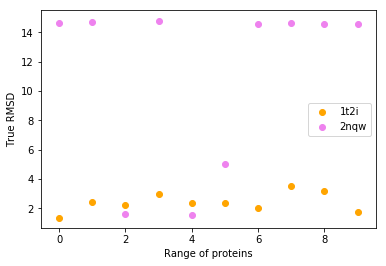
\includegraphics[width=0.5\textwidth]{images/relatorio/true_rmsd.png}
    \caption{Valor do RMSD para cada decoy no top 10. Não existem falsos mínimos para a proteína 1T2I, enquanto
    isso existem 7 falsos mínimos para a proteína 2NQW.}
    \label{fig:truermsd}
    \fautor
\end{figure}

\subsubsection{Resultados}

Para podermos comparar os resultados dos teste utilizando imagens de persistência, 
treinamos os mesmos algoritmos no conjunto de propriedades de proteínas dadas pelo \textit{Rosetta} 
quando desenvolvendo um novo decoy. As propriedades são dadas por
\begin{center}
    fa\_dun, fa\_elec, fa\_intra\_rep, hbond\_sc,

    fa\_rep, fa\_sol, hbond\_bb\_sc, hbond\_lr\_bb,

    hbond\_sr\_bb, omega, p\_aa\_pp, pro\_close, rama.
\end{center}
Quando treinamos os regressores com essas propriedades, obtemos as seguintes figuras. 
Na Figura~\ref{fig:res1t2i} são os resultados para a proteínas 1T2I e na Figura~\ref{fig:res2nqw} 
os resultados para 2NQW.

\begin{figure}[!htbp]
    \centering
    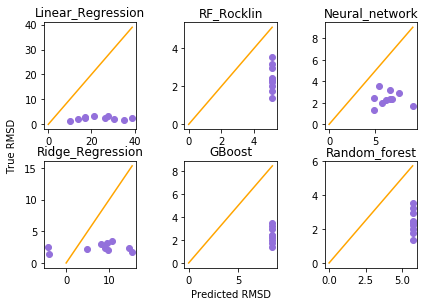
\includegraphics[width=.7\linewidth]{images/relatorio/res1t2i.png}
    \caption{Proteína 1T2I. RMSD previsto x RMSD verdadeiro para o top 10 dados os 
             regressores treinados em outras proteínas.}
    \label{fig:res1t2i}
    \fautor
\end{figure}

\begin{figure}[!htbp]
    \centering
    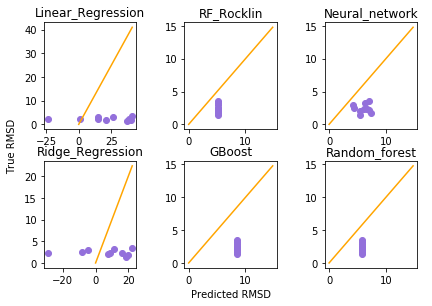
\includegraphics[width=.7\linewidth]{images/relatorio/res2nqw.png}
    \caption{Proteína 2NQW. RMSD previsto x RMSD verdadeiro para o top 10 dados os 
             regressores treinados em outras proteínas.}
    \label{fig:res2nqw}
    \fautor
\end{figure}

Agora podemos analisar os modelos que utilizam imagens de persistência no treinamento. Na 
Tabela~\ref{tab:run_numb} temos
os parâmetros utilizados para diversos testes. A coluna \textbf{Pixel} mostra o tamanho das imagens, $n$
signifca $(n,n)$. \textbf{\# Teste} é uma identificação para os resultados. Para cada teste três diagramas
de persistência foram calculados, somente os átomos C-$\alpha$, os átomos N e O e por fim todos os átomos
menos os de hidrogênio.

\begin{table}[!htbp]
    \centering
    \caption{Alguns dos testes feitos para obter as imagens de persistência e usa-las para o
             treinamento.}
    \label{tab:run_numb}
    \begin{tabular}{@{}cccc@{}}
    \toprule
    \textbf{\# Teste} & \textbf{Pixel} & \textbf{Variância} & \textbf{Dimensão PD} \\
    \midrule
    1                   & 10                  & 0,3             & 1                     \\
    2                   & 10                  & 0,5             & 1                     \\
    3                   & 10                  & 0,6             & 1                     \\
    4                   & 10                  & 0,8             & 1                     \\
    5                   & 10                  & 1,0             & 1                     \\
    6                   & 10                  & 1,2             & 1                     \\
    7                   & 3                   & 1,0             & 1                     \\
    8                   & 5                   & 1,0             & 1                     \\
    9                   & 50                  & 0,3             & 1                     \\
    10                  & 50                  & 1,0             & 1                     \\
    11                  & 100                 & 0,3             & 1                     \\
    12                  & 100                 & 1,0             & 1                     \\
    %18                  & 6                   & 0.3             & 1                     \\
    %19                  & 6                   & 0.5             & 1                     \\
    %20                  & 6                   & 0.6             & 1                     \\
    %21                  & 6                   & 0.8             & 1                     \\
    %22                  & 6                   & 1.0             & 1                     \\
    %23                  & 6                   & 1.2             & 1                     \\
    %24                  & 8                   & 0.3             & 1                     \\
    %25                  & 8                   & 0.5             & 1                     \\
    %26                  & 8                   & 0.6             & 1                     \\
    %27                  & 8                   & 0.8             & 1                     \\
    %28                  & 8                   & 1.0             & 1                     \\
    %29                  & 8                   & 1.2             & 1                     \\
    \bottomrule
\end{tabular}
\end{table}

Treinamos os mesmos regressores como anterioemnte para varias proteínas. Definimos então $4$ métricas diferentes
para selecionar o melhor regressor com respeito a cada uma. As métricas são:
\begin{itemize}
    \item $R^2$ score: medida estatística para medir o quão perto os dados estão da linha de regressão;
    \item MSE: Erro quadrático médio;
    \item RMSE: Raíz do erro quadrático médio;
    \item Acurácia binária: Converte cada RMSD para 0 ou 1 usando a seguinte regra: se o RMSD é maior que
          $5$ então 0, senão 1.
\end{itemize}

A Tabela~\ref{tab:bestruns} mostra os melhores experimentos para cada métrica usando imagens de persistência na hora do treinamento.
\begin{table}[!htbp]
    \centering
    \caption{Melhores parâmetros para cada métrica para os regressores treinados nas imagens de persistência.}
    \label{tab:bestruns}
    \begin{tabular}{@{}cccccc@{}}
    \toprule
    \textbf{Métrica} & \textbf{Regressor} & \textbf{Pixel} & \textbf{Variância} &
    \textbf{Lista de átomos}\footnote{Atomos utilizados para calcular os diagramas de persistência. "todo" significa
    que todos os átomos menos os de hidrogênio foram usados para os PD's.}
     & Score médio
    \\
    \midrule
    $R^2$           & Redes neurais     & 100       & 1,0             & C     & $-5,780$ \\
    MSE             & Redes neurais     & 100       & 1,0             & C     &  $8,299$  \\
    RMSE            & Regressão lin c/ reg.   & 10    & 1,2           & todo  &  $2,599$  \\
    Acurácia Binária & GBoost             & 10      & 0,6             & N,O   &  $0,657$  \\
    \bottomrule
    \end{tabular}
\end{table}
Por outro lado, a Tabela~\ref{tab:rosregr} mostra os melhores regressores treinados 
nas propriedades dadas pelo \textit{Rosetta}. 
\begin{table}[!htbp]
    \centering
    \caption{Melhores regressores treinados com as propriedades das proteínas}.
    \label{tab:rosregr}
    \begin{tabular}{@{}ccc@{}}
        \toprule
        \textbf{Métrica} & \textbf{Regressor} & \textbf{Score médio} \\ \midrule
        $R^2$           & Random Forest II       &-13,706        \\
        MSE             & Random Forest II       & 10,113         \\
        RMSE            & Random Forest II        & 2,707          \\
        Acurácia binária & Regressão lin. c/ reg. & 0,586          \\ \bottomrule
    \end{tabular}
\end{table}

Os regressores treinados com imagens de persistência obtiveram melhores resultados 
do que os treinados utilizando as propriedades que o \textit{Rosetta} para todas as métricas.
Podemos ver na Figura~\ref{fig:1t2i_binary} e ~\ref{fig:2nqw_binary} que os modelos baseados em 
imagens de persistência possuem uma maior acurácia binária. O método baseado em propriedades topológicas
pode ser estendido. Devido a sua natureza e similaridade com imagens, pode-se utilizar redes neurais 
convolucionais para o treinamento. 
\begin{figure}[!htbp]
    \centering
    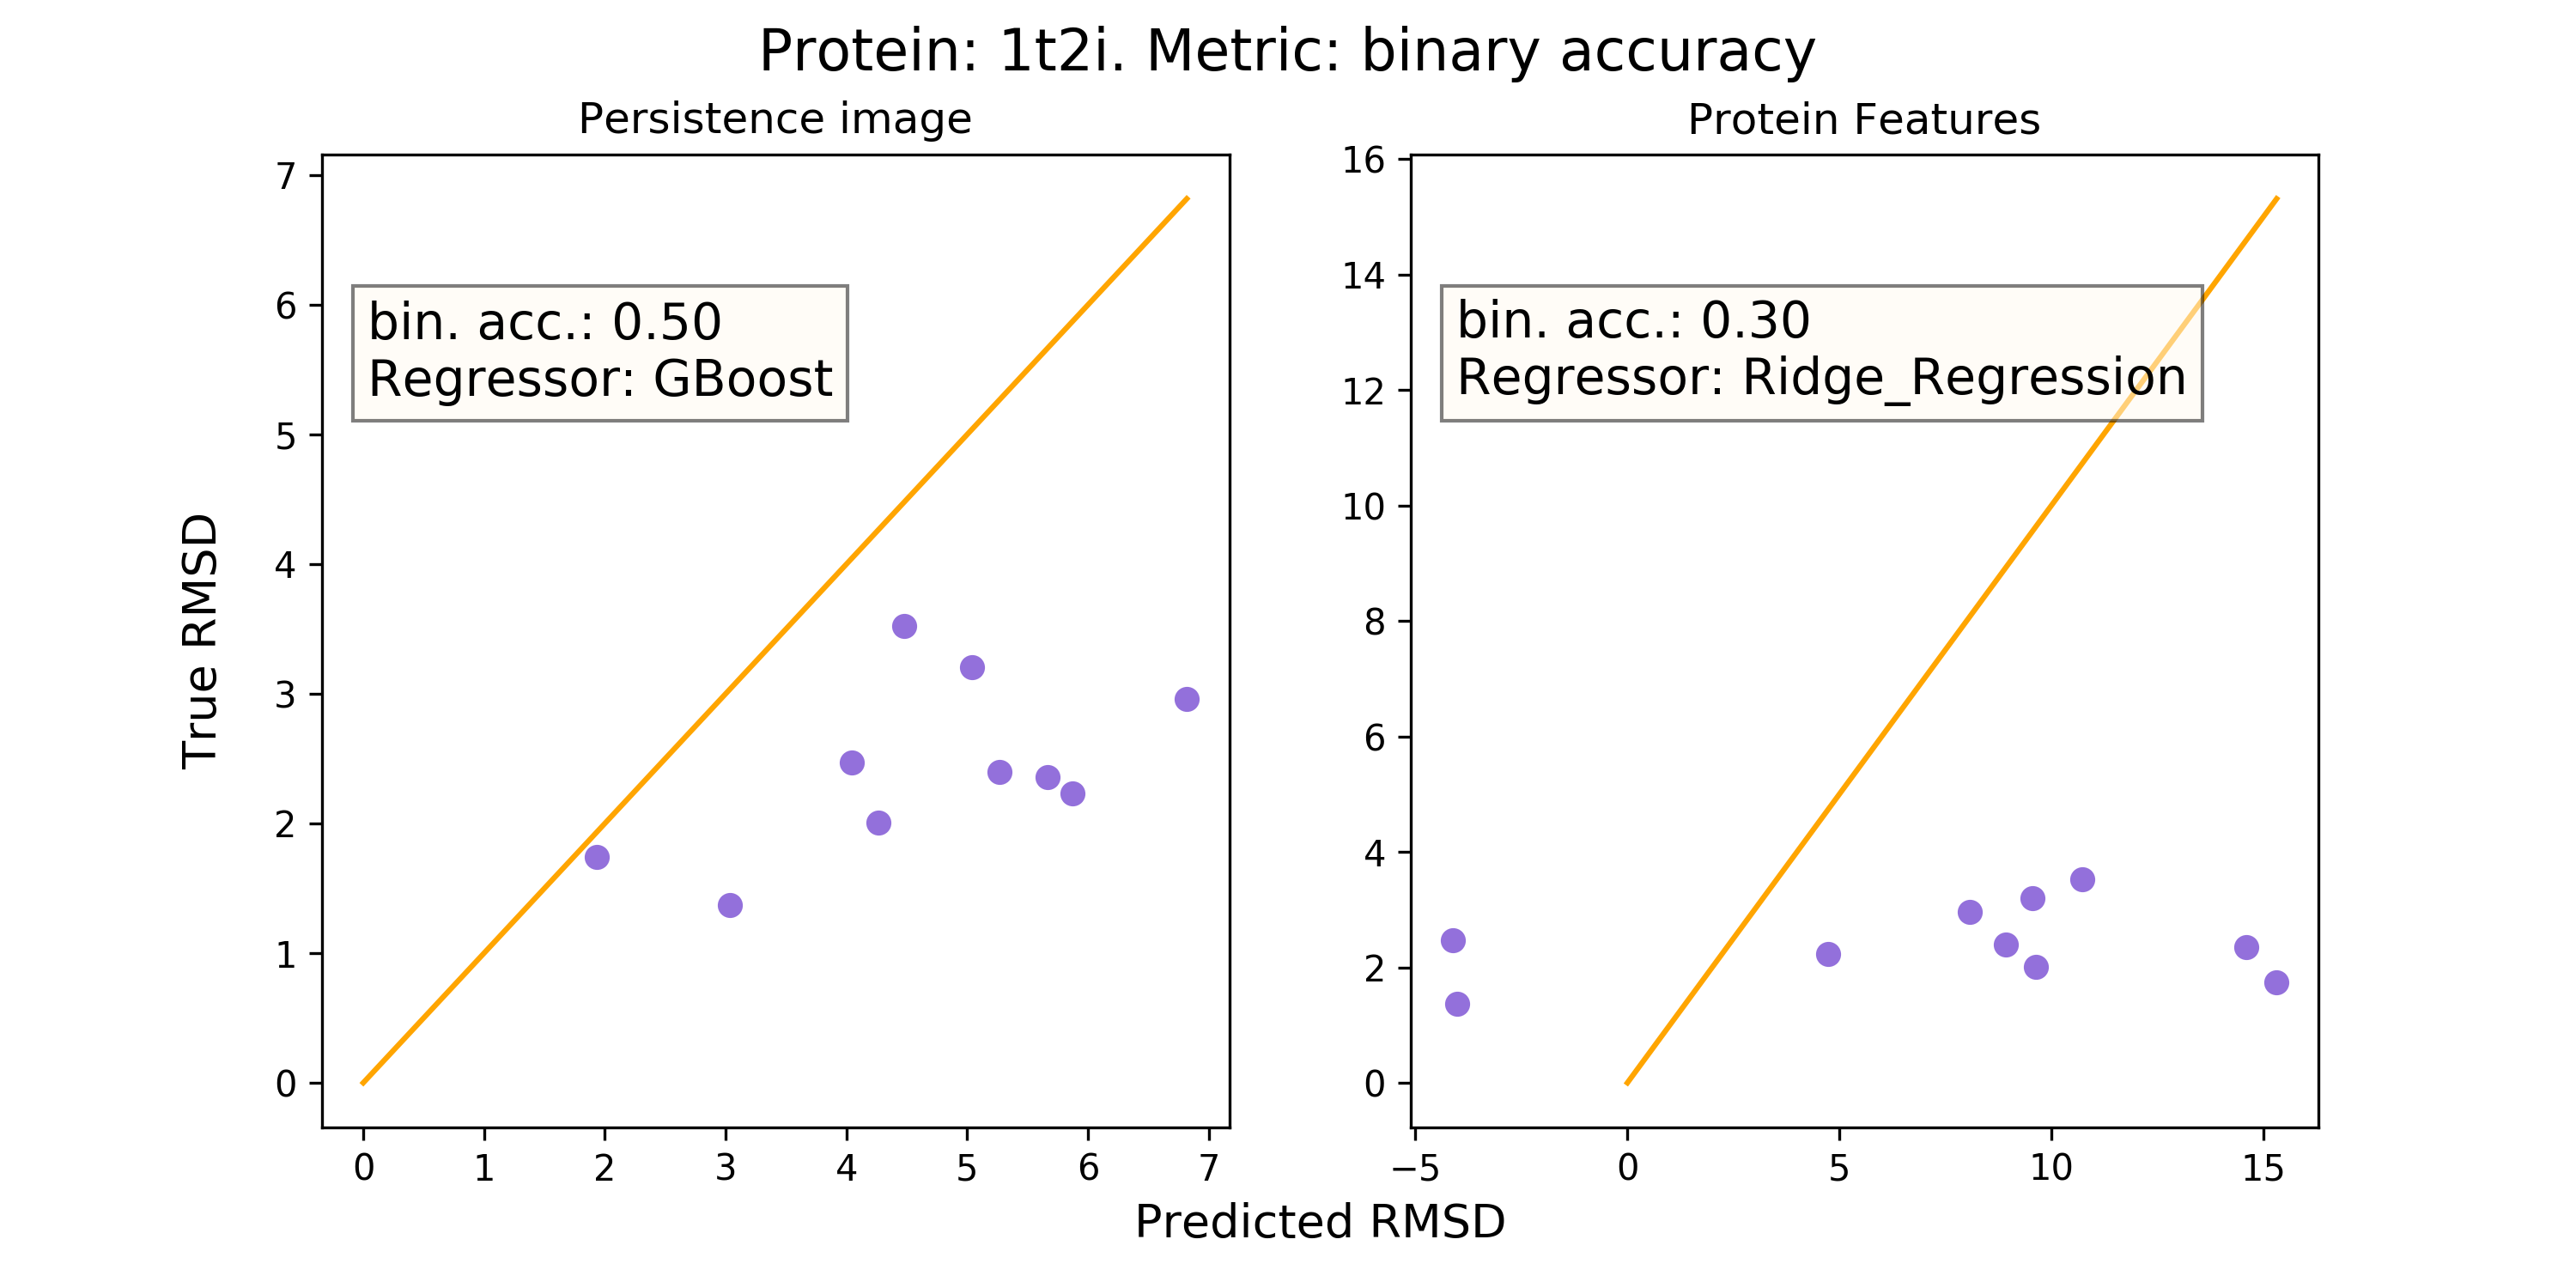
\includegraphics[width=0.99\textwidth]{images/relatorio/1t2i_binary.png}
    \caption{RMSD previsto x RMSD verdadeiro para o top 10 decoys da proteína 1T2I dados os 
             regressores com a melhor acurácia binária no conjunto de validação.}
    \label{fig:1t2i_binary}
    \fautor
\end{figure}

\begin{figure}[!htbp]
    \centering
    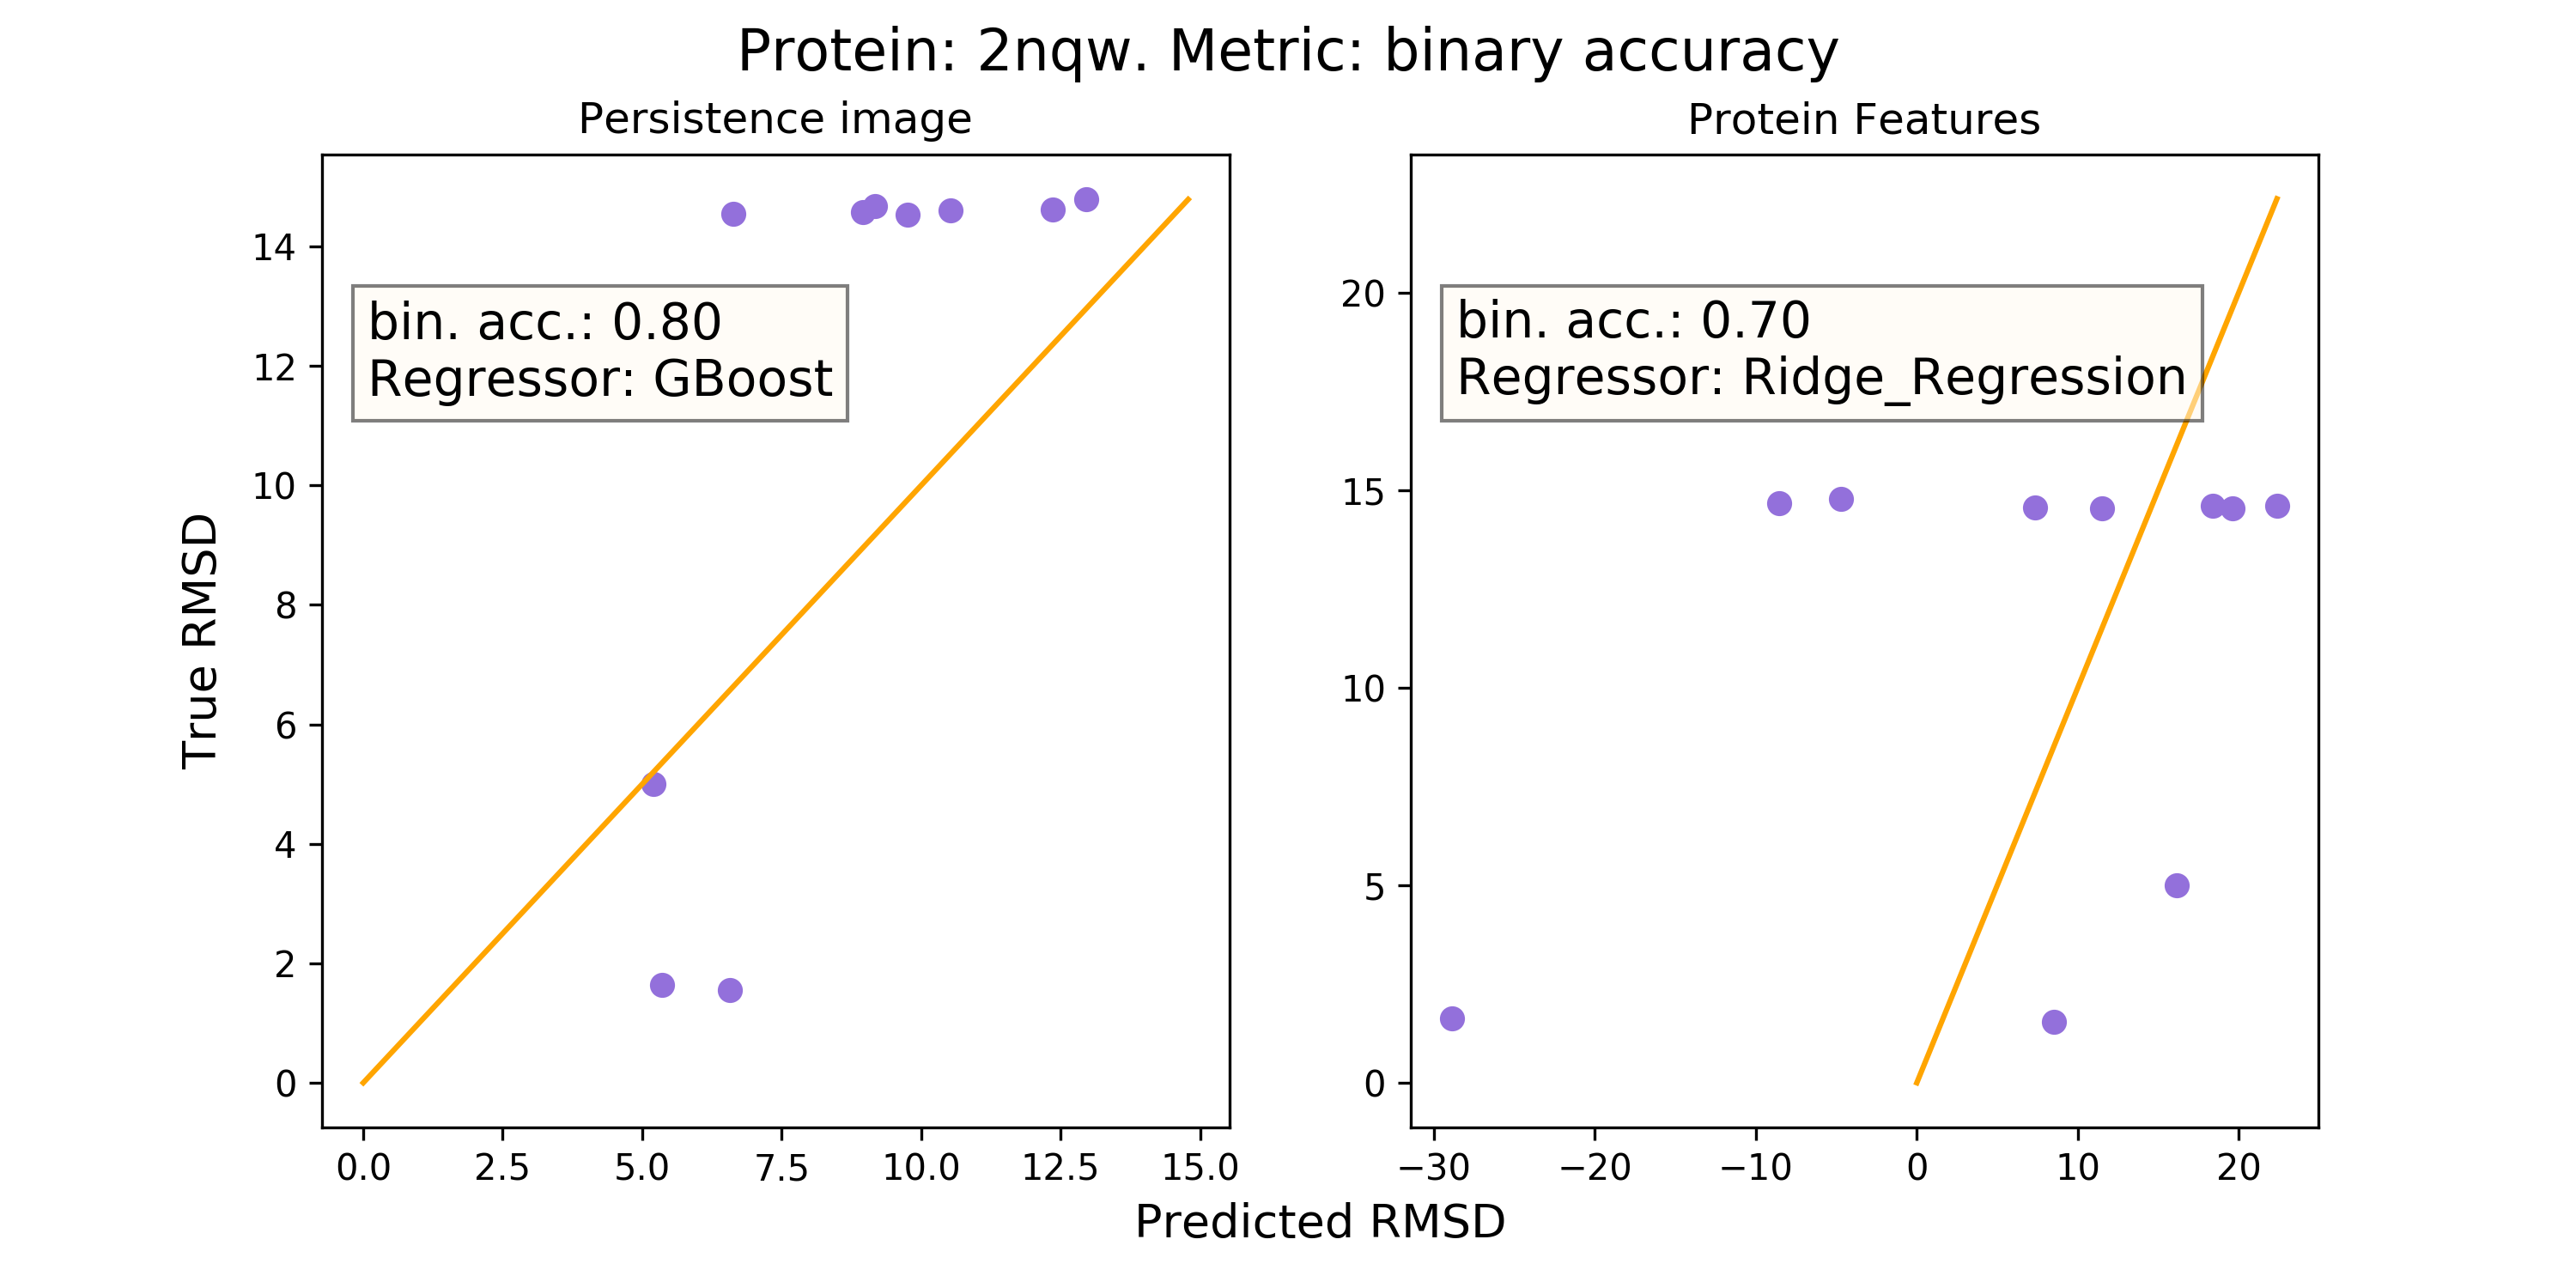
\includegraphics[width=0.99\textwidth]{images/relatorio/2nqw_binary.png}
    \caption{RMSD previsto x RMSD verdadeiro para o top 10 decoys da proteína 2NQW dados os 
             regressores com a melhor acurácia binária no conjunto de validação.}
    \label{fig:2nqw_binary}
    \fautor
\end{figure}

Este trabalho mostra que usar imagens de persistência é melhor para as tarefas de predição do RMSD
para proteínas não vistas anteriormente. Os algortimos treinados podem ser usados como uma função
para o \textit{Rosetta} utilizar na hora dos passos de minimização no desenvolvimento de novas proteínas.

O Jupyter Notebook \cite{Kluyver2016} está disponível online com a lista completa de proteínas (ID's) utilizadas 
no treinamento e teste, assim como com o código para a análise de resultados dos modelos. Os arquivos
podem ser baixados \href{https://drive.google.com/file/d/160DZgRiPwsHNaTzasQxd2VaIXCUkiLZG/view?usp=sharing}{aqui}
(\url{https://bit.ly/2XUjat2}).

